\chapter{Kinematic Equations}

Considering the UAV as a rigid body, the standard kinematic equations will be used. Due to the scope of this analysis, the \textbf{Flat-Earth model} equations will be used, instead of a round Earth (eg WGS-84 model). This option was made since the intended UAV area of operations will be constrained over a small area. GPS coordinates will be used as in a Cartesian grid.

\section{Position}

We express the position vector as
\begin{equation} \label{eq:navshort}
	\bm{p} = [n\ e\ d]^T
\end{equation}
The variables $n$, $e$ and $d$ correspond to the North, East and Down direction, which constitute the primary axis of the NED (as it is called) coordinate system. We shall denote this frame as $\mathcal{F}_F$. The origin of the NED frame is arbitrarily located at the home of operations (or launch point) of every mission and placed on the surface of the Eearth.
In contrast, the origin of the so-called body-axes $\mathcal{F}_B$ is the center of gravity point of the aircraft. Its x-axis is placed on the line of longitudinal symmetry, its y-axis starboard and the z-axis downwards, producing a right-handed frame, which can be seen in the following figure.

\begin{figure}[H]
\centering
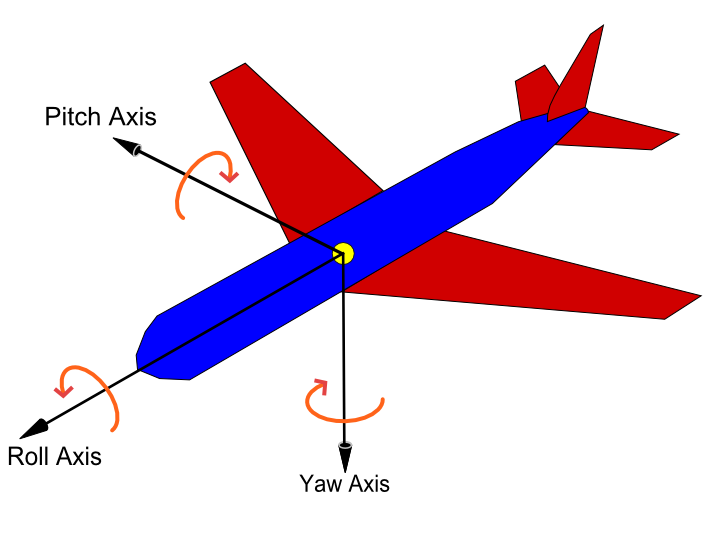
\includegraphics[width=0.45\linewidth]{Figures/Plane_Axes}
\caption{Aircraft body axes}
\label{fig:Plane_Axes}
\end{figure}


The derivative of the position is
\begin{IEEEeqnarray}{rCl} \label{eq:posDot}
	\dot{\bm{p}} &= & \bm{R}_b^T \bm{v_b}
\end{IEEEeqnarray}
We denote with $R_b$ the transformation matrix \textbf{from the Inertial frame to the Body frame}. Its elements are:

\begin{equation}
\bm{R}_b = \begin{bmatrix}
	\cos \theta \cos \psi                             & \cos\theta \sin\psi                               & -\sin\theta         \\
	-\cos\phi \sin\psi + \sin\phi \sin\theta \cos\psi & \cos\phi \cos\psi + \sin\phi \sin\theta\sin\psi   & \sin\phi \cos\theta \\
	\sin\phi \sin\psi + \cos\phi \sin\theta \cos\psi  & -\sin\phi \cos\psi + \cos\phi \sin\theta \sin\psi & \cos\phi \cos\theta
\end{bmatrix}
\end{equation}


Equation \eqref{eq:posDot} can be broken down onto its three elements as
\begin{IEEEeqnarray}{rCl}
	\dot{n} &= &(\cos \theta \cos \psi) u + (-\cos\phi \sin\psi + \sin\phi \sin\theta \cos\psi) v \nonumber\\
	&& +\> (\sin\phi \sin\psi + \cos\phi \sin\theta \cos\psi)w \IEEEyessubnumber \\
	\dot{e} &= & (\cos\theta \sin\psi)u + (\cos\phi \cos\psi + \sin\phi \sin\theta\sin\psi)v  \nonumber\\
	&& +\> (-\sin\phi \cos\psi + \cos\phi \sin\theta \sin\psi)w \IEEEyessubnumber \\
	\dot{d} &= & (-\sin\theta)u + (\sin\phi \cos\theta)v + (\cos\phi \cos\theta)w \IEEEyessubnumber
\end{IEEEeqnarray}

We see that the rotation matrix $\bm{R_B}$ is dependent upon three variables, $\phi$ , $\theta$ and $\psi$ . These are explained below.

\section{Orientation}

We use Euler angle notation to express the orientation of the aircraft. Roll, pitch and yaw are denoted as $\phi$, $\theta$ and $\psi$ respectively.
\begin{equation}
	\bm{\Phi} = [\phi \ \theta \ \psi]^T
\end{equation}

Figure \ref{fig:Euler_Anlges_2} has a visual representation of those angles. Take a note at the order of rotations: the standard order for aircraft applications, in order to come up with the body frame $\mathcal{F}_B$, starting from the NED frame is:
\begin{enumerate}
\item Rotate around NED z-axis by angle $\psi$, producing frame $\mathcal{F}_1$
\item Rotate around $\mathcal{F}_1$ y-axis by angle $\theta$, producing frame  $\mathcal{F}_2$
\item Rotate around  $\mathcal{F}_2$ x-axis by angle $\phi$, producing the $\mathcal{F}_B$ frame
\end{enumerate}
This convention is called the \emph{Tait-Bryan angles} \cite{Berner2008}

\begin{figure}[H]
\centering
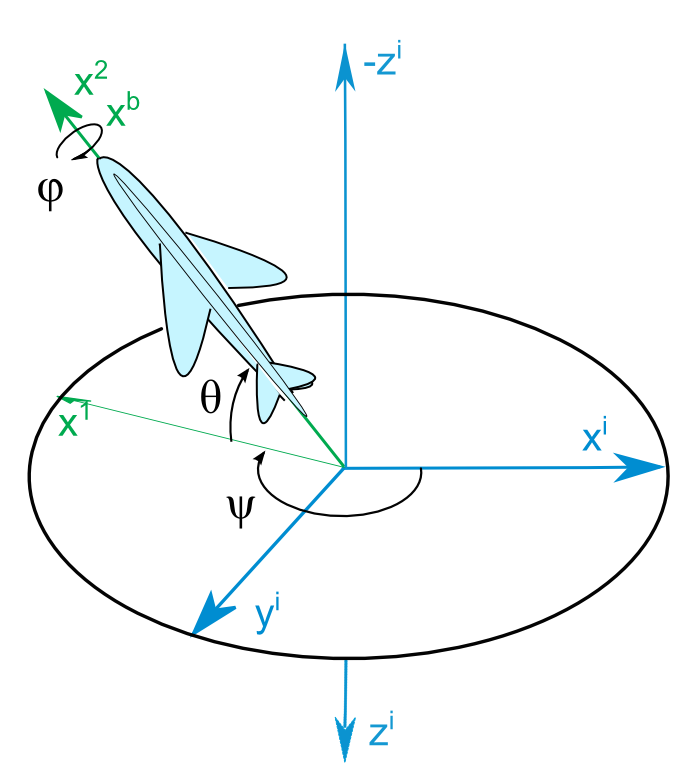
\includegraphics[width=0.35\linewidth]{Figures/Euler_Anlges_2}
\caption{Euler angles}
\label{fig:Euler_Anlges_2}
\end{figure}


The time derivative of the Euler angles is
\begin{equation}
	\dot{\bm{\Phi}} = \mathcal{E}(\bm{\Phi})\bm{\omega_b}
\end{equation}
where $\mathcal{E}(\bm{\Phi})$ is a rotation matrix, dependent upon the current orientation.

The individual angle propagation equations are
\begin{IEEEeqnarray}{rCl}
	\dot{\phi} & = & p + \tan\theta \sin\phi q + \tan\theta \cos\phi r \IEEEyessubnumber \\
	\dot{\theta} &= & \cos\phi q - \sin\phi r \IEEEyessubnumber \\
	\dot{\psi} &= & \frac{\sin\phi}{\cos\theta} q + \frac{\cos\phi}{\cos\theta} r \IEEEyessubnumber 
\end{IEEEeqnarray}

and equivalenty, $ \mathcal{E}(\bm{\Phi})$ is written as
\begin{equation}
\mathcal{E}(\bm{\Phi}) = \begin{bmatrix}
	1 & \tan \theta \sin \phi        & \tan \theta \cos \phi       \\
	0 & \cos \phi                    & -\sin \phi                  \\
	0 & \frac{\sin\phi}{\cos\theta} & \frac{\cos\phi}{\cos\theta}
\end{bmatrix}
\end{equation}

\section{Angular velocity}

We define the angular velocity vector as
\begin{equation}
	\bm{\omega} = [p\ q\ r]^T
\end{equation}

and its time derivative is
\begin{equation}  \label{eq:angVelDer}
	\dot{\bm{\omega}} = \frac{1}{\bm{J}}\left(\bm{T_b} - \bm{\omega} \times (\bm{J} \bm{\omega_b})\right)
\end{equation}
This equation incorporates the inertia matrix $\bm{J}$ and the input torque, expressed in the body axes $T_b$.

By spreading out the lines of the above vector equation we get

\begin{IEEEeqnarray}{rCl}
	\dot{p} &= & \frac{1}{\Gamma} \left[J_{xz} (J_x - J_y + J_z)pq - (J_z(J_z-J_y)+J_{xz}^2)qr + J_z T_x + J_{xz}T_z\right] \IEEEyessubnumber \\
	\dot{q} &= & \frac{1}{J_y} \left[(J_z - J_x)pr - J_{xz}(p^2 - r^2)+ T_y\right] \IEEEyessubnumber \\
	\dot{r} &= & \frac{1}{\Gamma} \left[((J_x - J_y)J_x + J_{xz}^2)pq - J_{xz}(J_x - J_y + J_z)qr + J_{xz}T_x + J_x T_z\right] \IEEEyessubnumber
\end{IEEEeqnarray}

To facilitate the calculation of cross products we may use this identity:
\begin{equation}
	\bm{\omega}\times \bm{v} = \begin{bmatrix}
		0  & -r & p  \\
		r  & 0  & -p \\
		-q & p  & 0
	\end{bmatrix} \bm{v}
\end{equation}
Where $\bm{v}$ is an arbitrary vector. Similarly,
\begin{equation}
	\bm{\omega} \times (\bm{\omega} \times \bm{v}) = \begin{bmatrix}
		-r^2-q^2 & pq & pr \\
		pq & -p^2 -r^2 & qr\\
		pr & qr & -p^2-q^2
	\end{bmatrix} \bm{v}
\end{equation}

The inertia matrix is defined as
\begin{equation}
	\bm{J} =
	\begin{bmatrix}
		\int(y^2 + z^2)~dm & -\int xy~dm        & -\int xz~dm        \\
		-\int xy~dm        & \int(x^2 + z^2)~dm & -\int yz~dm        \\
		-\int xz~dm        & -\int yz~dm        & \int(x^2 + y^2)~dm
	\end{bmatrix}
\end{equation}
Commonly, the inertia matrix in fixed-wing aircraft is considered to have zero elements in the x-y and y-z direction, since they are symmetric about the x-z plane.
\begin{equation}\label{eq:inertiaMat}
	\bm{J} = 
	\begin{bmatrix}
		J_x     & 0   & -J_{xz} \\
		0       & J_y & 0       \\
		-J_{xz} & 0   & J_z
	\end{bmatrix}
\end{equation}
	
\begin{equation}
	\Gamma = J_x J_z - J_{xz}^2
\end{equation}


\section{Linear Velocity}

We define linear velocity and its components as
\begin{equation}
	\bm{v_b} = [u\ v\ w]^T
\end{equation}

Its time derivative is
\begin{equation}
	\dot{\bm{v_b}} = -\bm{\omega_b} \times \bm{v_b} + \frac{\bm{F_b}}{m}
\end{equation}

which is equivalent to
\begin{IEEEeqnarray}{rCl}
	\dot{u} &= & rv -qw + \frac{F_bx}{m} \IEEEyessubnumber \\
	\dot{v} &= & -ru + pw + \frac{F_by}{m} \IEEEyessubnumber \\
	\dot{w} &= & qu -pv + \frac{F_bz}{m} \IEEEyessubnumber
\end{IEEEeqnarray}

We need to define the wind velocity, in the body frame. This is the velocity of the air-mass, moving above the ground, expressed in the body axes.
\begin{equation}
	\bm{v_w} = [u_w\ v_w\ w_w]^T
\end{equation}

The resulting relative (air)speed of the aircraft is
\begin{equation}
	\bm{v_r} = \bm{v}_B - \bm{v}_w
\end{equation}

Relative velocity is a very important quantity in aeronautics, as every aspect of the aircraft's aerodynamic response depends on it, rather than the inertial speed.

Based on the relative velocity, we define three more quantities:
\begin{itemize}
\item the angle of attack, $\alpha$
\item the angle of sideslip, $\beta$
\item the airspeed, $V_a$
\end{itemize}


\begin{IEEEeqnarray}{rCl}
	\alpha &= &\tan^{-1} \left(\frac{w_r}{u_r}\right) \IEEEyesnumber \IEEEyessubnumber \\
	\beta &= &\sin^{-1}\left(\frac{v_r}{V_a}\right) \IEEEyessubnumber \\
	V_a &= &\lVert[u_r\ v_r\ w_r]^T\rVert
\end{IEEEeqnarray}

Using these angles, a new frame of reference can be constructed, the Stability frame $\mathcal{F}_S$. The relative speed components (expressed in the body frame) can be constructed from the airspeed (expressed in the stability frame) using the following rotation:

\begin{equation}
\bm{v}_r = \bm{S}^T \begin{bmatrix}
V_a \\ 0 \\ 0
\end{bmatrix}
\end{equation}

\begin{equation}\label{eq:StabMatrix}
	\bm{S}=
	\begin{bmatrix}
		\cos\alpha \cos\beta & \sin\beta & \sin\alpha \cos\beta \\
		-\cos\alpha \sin\beta & \cos\beta & -\sin\alpha \sin\beta \\
		-\sin\alpha & 0 & \cos\alpha
	\end{bmatrix}
\end{equation}



\section{Mass Distribution}

It is useful to model the mass distribution of our aircraft. It has a nominal mass $m_{nom}$, placed at the center of gravity, the origin of the body axes. Any extra weights, such as payloads, debris, or component detachment can be modeled with extra masses $m_i$. Under this definition, $m_i$ is allowed to be negative.

\begin{IEEEeqnarray}{rCl}\label{eq:masses}
	m &= & m_{nom} + \sum m_i \IEEEyesnumber \IEEEyessubnumber \\
	\bm{p}_{m,nom} &= &[0\ 0\ 0]^T \IEEEyessubnumber \\
	\bm{p}_{CG} &= & \frac{1}{m} \left( \sum \bm{p}_i m_i\right)
\end{IEEEeqnarray}

Naturally, mass additions also affect the matrix of inertia of the aircraft. A mass $m_{e}$ planed at the point $p_{e} = [x_{e}, y_{e}, z_{e}]^T$ perturbs the matrix of inertia by
\begin{equation}
	\Delta \bm{J} =
	\begin{bmatrix}
		y_{e} z_{e} m_{e}  & -x_{e} y_{e} m_{e} & -x_{e}z_{e}m_{e}   \\
		-x_{e} y_{e} m_{e} & x_{e} z_{e} m_{e}  & -y_{e} z_{e} m_{e} \\
		-x_{e}z_{e}m_{e}   & -y_{e} z_{e} m_{e} & x_{e} y_{e} m_{e}
	\end{bmatrix}
\end{equation}
However, this perturbation in the matrix of inertia has not been incorporated into the angular velocity derivatives equations (\ref{eq:angVelDer}), for reasons of simplicity. 

\section{Wind Disturbances}
Another interesting model, primarily for simulation of autopilot software, is the one describing wind disturbances. It incorporates two sub-models: one for describing the constant wind velocity, as a function of altitude and one for producing wind turbulence. Static wind is intuitively expressed in the inertial frame, while turbulence is usually expressed in the body frame, so care is required in order to avoid confusion and errors in notation and coding.

\begin{equation}
	\bm{v_w} = \bm{v_{ws}} + \bm{v_{wg}}
\end{equation}

We denote with $\bm{v_{ws}}$ the constant wind vector, with components.

\begin{equation}
\bm{v_{ws}} = \bm{R}_B^T[v_{ws,n}, v_{ws,e}, v_{ws,d}]^T
\end{equation}

Usually we consider the vertical component of the wind to be zero ($v_{ws,d}=0$)

Another useful expression for constant wind is:
\begin{equation}
\bm{v_{ws}} = \bm{R}_B^TV_{ws}[-\cos\theta_w, -\sin\theta_w, 0]^T
\end{equation}
where $V_{ws}$ is the wind overall magnitude (in $m/s$) and $\theta_w$ is the wind direction (0degrees for North wind)

This allows us to introduce an altitude model for the wind magnitude, commonly known as the Power Law:
\begin{equation}
V_{ws} = V_{ws,h_r} \left(\frac{h}{h_r}\right)^\alpha
\end{equation}
This formula describes the increase of the wind magnitude as an exponential function of the altitude, given a measurement of wind magnitude $V_{ws,h_0}$ at altitude $h_0$. $\alpha$ is the Hellmann exponent (roughness exponent), which describes the wind shear effect. Commonly, surface wind magnitude measurements are available for the altitude of 10m, so the above formula becomes.
\begin{equation}
V_{ws} = V_{ws,h_10} \left(\frac{h}{h_10}\right)^\alpha
\end{equation}

Values for $\alpha$ vary with terrain morphology and wind turbulence. Some indicative values can be found in references \cite{Banuelos-Ruedas2011}, \cite{Peterson1978}, \cite{wiki:WindGrad}, \cite{wiki:Wind_profile_power_law}, but it is also claimed that the "1/7th power law" (using a value $\alpha=1/7$) is an adequate approximation for most purposes.
It should be noted, however, that most of the reviewed studies where oriented towards wind farm applications and wind models where validated up to a few hundred meters above ground.

The following table is pulled from \cite{Banuelos-Ruedas2011}

\begin{table}[H]
\centering
\begin{tabular}{|c|c|}
	\hline
	           Landscape type             & Friction coefficient $\alpha$ \\ \hline
	 Lakes, ocean and smooth hard ground  &              0.1              \\ \hline
	      Grasslands (ground level)       &             0.15              \\ \hline
	    Tall crops, hedges and shrubs     &             0.20              \\ \hline
	        Heavily forested land         &             0.25              \\ \hline
	Small town with some trees and shrubs &              0.3              \\ \hline
	 City areas with high rise buildings  &              0.4              \\ \hline
\end{tabular} 
\caption{Hellmann Exponent Values over Various Terrain}
\end{table}

An alternative model for wind shear can be found in \cite{Moorhouse1982}

Wind gusts can be modeled using Dryden transfer functions, as presented in \cite{Moorhouse1982}, \cite{BEAL1993}, \cite{MathWorks:DrydenTurbulence} and \cite{Beard2012} . Time responses can be generated by feeding unit variance white noise in the following filters. Note that airspeed is a parameter for these functions, but it can be replaced with the mean or cruise airspeed of the aircraft.
\begin{equation}
	\bm{V_{wg}}(s) =
	\begin{bmatrix}
		\sigma_u \sqrt{\frac{2V_a}{\pi L_u}} \frac{1}{s + \frac{V_a}{L_u}}\\
		\sigma_v \sqrt{\frac{3V_a}{\pi L_v}} \frac{s+\frac{V_a}{\sqrt{3}L_v}}{(s+\frac{V_a}{Lu})^2} \\
		\sigma_w \sqrt{\frac{3V_a}{\pi L_w}} \frac{s+\frac{V_a}{\sqrt{3}L_w}}{(s+\frac{V_a}{L_w})^2}
	\end{bmatrix}
\end{equation}

% Read BEAL1993 and verify the results

Typical values for the transfer function parameters for a small UAV can be found in \cite{Langelaan2011} and are copied below.
\begin{table}[H]
\centering
\begin{tabular}{|p{5cm}|c|c|c|c|c|}
	\hline
	            Description              & altitude (m) & $L_u$ (m) & $L_w$  (m) & $\sigma _u$ (m/s) & $\sigma _w$ (m/s) \\ \hline
	   low altitude, light turbulence    &      50      &    200    &     50     &       1.06       &       0.7        \\ \hline
	 low altitude, moderate turbulence   &      50      &    200    &     50     &       2.12       &       1.4        \\ \hline
	 medium altitude, light turbulence   &     600      &    533    &    533     &       1.5        &       1.5        \\ \hline
	medium altitude, moderate turbulence &     600      &    533    &    533     &       3.0        &       3.0        \\ \hline
\end{tabular} 
\caption{Gust Field Properties}
\end{table}